\documentclass{beamer}
\renewcommand{\baselinestretch}{1.1}
\usepackage{graphicx}
\usepackage{natbib}
\usepackage{amsmath}
\usepackage{hyperref}
\usepackage{listings} 

\def\labelitemi{--}
\parindent=0pt

\usepackage{xcolor}

\colorlet{codecolor}{black!30}
\newcommand{\codebox}[1]{%
  \colorbox{codecolor}{\ttfamily \detokenize{#1}}%
}

\begin{document}
\bibliographystyle{/Users/Lizzie/Documents/EndnoteRelated/Bibtex/styles/besjournals}
\renewcommand{\refname}{\CHead{}}

{\usebackgroundtemplate{%
  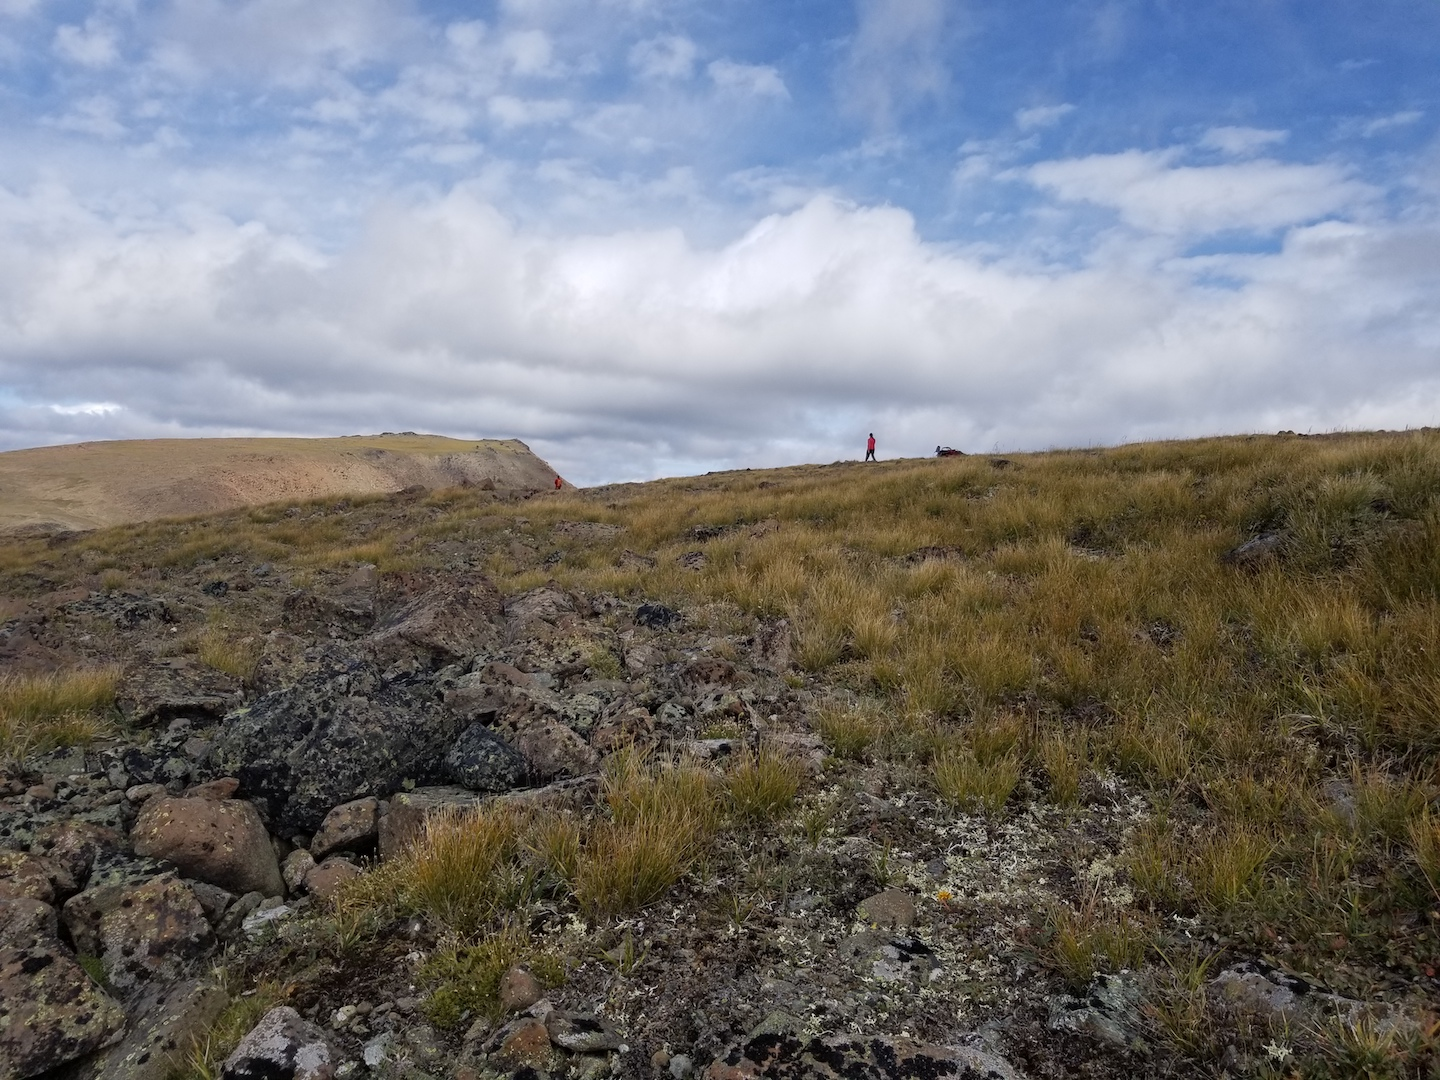
\includegraphics[width=\paperwidth,height=\paperheight]{photo.jpg}} 
\begin{frame}
\begin{center}
\vspace{20ex}
{\color{white} {\huge Phylogeny model updates}}
\\
\vspace{3ex}
{\color{white} {\Large 10 June 2020}}

\end{center}
\end{frame}
}
	
	\frame{
		\frametitle{What I will cover...}
		\framesubtitle{}
		\begin{itemize}
			\item The way phylogeny is generally handled in ecological statistical models
		\begin{itemize}
                  \item PGLS
                    \item PMM
		\end{itemize}
			\item The way I want to handle it for OSPREE (but I could be wrong)
			\item My progress on that goal
		\end{itemize}
	}

	\frame{
		\frametitle{A couple quick notes ... }
		\framesubtitle{}
		\begin{itemize}
			\item I am skipping over why we care about phylogeny, check out phylogenyfoundering.pdf for some of that.
                         \item Phylogenetic structure in a value (say, a `trait') is measured based on a value called $\lambda$. When $\lambda=1$ the trait is perfectly predicted by the phylogeny; when it's 0, the phylogeny does not matter. 
                           \item You can play with the code in ubermini.R or  max\_sims.R to get a feel for this.
		\end{itemize}
	}


	\frame{
		\frametitle{Common modeling approaches}
		\framesubtitle{Part 1: PGLS (adapted from second edition of \emph{Statistical Rethinking})}
Consider...
\begin{align}
y & \sim MVN(\mu, S)\\
\mu_i & = \alpha +  \beta*x_i
\end{align}
$\mu$ is a usual linear model. $P$ is a vector of phenological dates (one per species), and $S$ is a covariance matrix with as many rows and columns as species. In ordinary regression this takes the form:
\begin{align}
S = \sigma^2I
\end{align}
where I is just an identity matrix (all 1s) so we can ignore it. 
In PGLS we replace $S$ with the phylogenetic covariance matrix ($\Sigma$). 
	}


	\frame{
		\frametitle{Common modeling approaches}
		\framesubtitle{Part 1: PGLS}
{\bf You have to make sure of a few things}: 
\begin{itemize}
\item Phylogeny must go in as correlation matrix (this makes the diagonals 1s and the off-diagonals the correlation across species due to evolutionary history) and make sure the rows and columns are in the same order as the species will be ordered numerically.
\item This model forces the correlation structure you give it---it does not adjust the correlation structure at all. 
\end{itemize}
If you don't want to assume $\lambda=1$, then you need to estimate a value to multiply the matix by such that:
\begin{align}
S = \sigma^2(\Sigma*\lambda)
\end{align}
	}

	\frame{
		\frametitle{Common modeling approaches}
		\framesubtitle{Part 2: PMM (phylogenetic mixed model)}
{\bf Now PMM...} 

\begin{align}
y & = \alpha + \beta x + a + e\\
a & \sim normal(0, \sigma_P^2\Sigma)\\
e & \sim normal(0, \sigma_R^2I)\\
\text{PGLS: }y & \sim normal(\alpha + \beta x, \sigma_P^2\Sigma)
\end{align}
... where $\alpha$ is the intercept $\beta$ is the slope for the co-factor x, $a$ is the phylogenetic random effect, and $e$ is the residual error. This model estimated two variances: $V_P$ is the variance of the phylogenetic effect and $V_R$ is the residual error (environment effects, intraspecific variance, measurement error, etc.). %  The two last terms are assumed to be normally distributed, with $\Sigma$ as a phylogenetic correlation matrix , $I$ stands for the relevant identity matrix. 

}
	\frame{
		\frametitle{Common modeling approaches}
		\framesubtitle{Part 3: PMM vs PGLS}
\begin{itemize}
\item People often stay PGLS does not allow for non-phylogenetically structured error (but I think it sort of does once you scale the phylogenetic effect by $\lambda$, no?) 
\item PMM explicitly models other sources of error through $e$.
\end{itemize}
In PMM the strength of the phylogenetic effect is measured as:

\begin{align}
\lambda & = \frac{\sigma^2_P}{\sigma^2_P+\sigma^2_R}
\end{align}
which is equivalent to just saying `what proportion of the variance is due to phylogeny?' 
	
	}

	\frame{
		\frametitle{What's wrong with this model?}
		\framesubtitle{What I want for OSPREE}
{\bf What is wrong with this?}
\begin{align}
y & = \alpha_0 + \alpha + \beta x + e\\
\alpha & \sim MVN(0, \sigma_{P\alpha}^2)\\
\beta & \sim MVN(0, \sigma_{P\beta}^2)\\
e & \sim normal(0, \sigma_y^2)\\
\sigma_{P\alpha}^2 & = \alpha_{\alpha} + \lambda_\alpha*\Sigma\\
\sigma_{P\beta}^2 & = \alpha_{\beta} + \lambda_\beta*\Sigma
\end{align}
Where $\alpha_0 $ is a grand mean and species-level intercepts are partially pooled by phylogeny, scaled by $\lambda_\alpha$ and slopes are also are partially pooled by phylogeny, scaled by $\lambda_\beta$, and there is some residual error $\sigma_y$.
	}

	\frame{
		\frametitle{What's wrong with this model?}
		\framesubtitle{What I want for OSPREE}
{\Large Did we answer `What's wrong with this model?'} \\
If not, go back, discuss.
	}


	\frame{
		\frametitle{What's wrong with this model?}
		\framesubtitle{What I want for OSPREE}
{\Large Also, I have another question....} \\
In linear regression like this, what's the difference between error and an intercept?
	}

	\frame{
		\frametitle{Where am I at?}
		\framesubtitle{What I have done}
		\begin{itemize}
			\item I have stolen code from Will Pearse, which he tells me should work.
                          \item I have it running for forcing, chilling, photo slopes... with the real OSPREE data, but it does not want to have phylogeny on the intercepts also (I want to try it with non-partially pooled intercepts ...).
\item I tried to do fake data
\item And now I am stuck ... (see ubermini.R and ubermini.stan)
		\end{itemize}
	}



	\frame{
		\frametitle{Where I am at}
		\framesubtitle{I am stuck}

The new code is this line I stole from Will Pearse's code:\\
\vspace{3ex}
bforce $\sim$  MVN(rep.vector(0,n.sp), \\
diag.matrix(repector(null.interceptsb, n.sp)) + lam.interceptsb$*$Vphy);\\

	}


	\frame{
		\frametitle{Where I am at}
		\framesubtitle{I am stuck}
bforce $\sim$  MVN(rep.vector(0,n.sp), \\
diag.matrix(repector(null.interceptsb, n.sp)) + lam.interceptsb$*$Vphy);\\
\vspace{3ex}
It says that my vector of slopes is multinormal centered around 0 (why zero? That's how Gaussian processes work, it somehow gets the `centering' if you will from the $y \sim normal(\hat{y}, \sigma_y)$ bit of the model) and the variance should be the within-species variance on the diagonal, and the between-species variance on the off-diagonals. 

	}



	\frame{
		\frametitle{Where I am at}
		\framesubtitle{I am stuck}

Let $\alpha$ be  null.interceptsb and $\lambda$ be lam.interceptsb.\\
\vspace{3ex}
bforce = 
\begin{equation*}
 \begin{bmatrix}
  \alpha+\lambda*Vphy &  \cdots & \lambda*Vphy \\
   & \ddots \\
  \lambda*Vphy & \cdots &   \alpha+\lambda*Vphy
 \end{bmatrix}
\end{equation*}
	}




	\frame{
		\frametitle{Where I am at}
		\framesubtitle{I am stuck}
If $Vphy$ is set to have 1s down the diagonal, we can simplify to this:\\
\vspace{3ex}
bforce = 
\begin{equation}
 \begin{bmatrix}
  \alpha+\lambda &  \cdots & \lambda*Vphy \\
   & \ddots \\
  \lambda*Vphy & \cdots &   \alpha+\lambda
 \end{bmatrix}
\end{equation}
	}


	\frame{
		\frametitle{Where I am at}
		\framesubtitle{I am stuck}
If $Vphy$ is set to have 0s down the diagonal, we can simplify to this:\\
\vspace{3ex}
bforce  = 
\begin{equation}
 \begin{bmatrix}
  \alpha &  \cdots & \lambda*Vphy \\
   & \ddots \\
  \lambda*Vphy & \cdots &   \alpha
 \end{bmatrix}
\end{equation}

\vspace{3ex}
This seems good---now the within-species estimate is $\alpha$ and the between-species is $\lambda*Vphy$.

	}



	\frame{
		\frametitle{}
		\framesubtitle{}
{\bf \Large And the crowd goes wild!}
	}


	\frame{
		\frametitle{No, just kidding}
		\framesubtitle{It's not working}
		\begin{itemize}
			\item I can return the slopes
\item $\lambda$ is wrong and I don't know why.
\item Any ideas? I have a tried a few things ... 
		\begin{itemize}
                  \item Set nind to 1 (1 value per species) .... no dice.
                    \item Tried taking it off slopes and putting on intercepts ... no dice.
                      \item Your idea here?
		\end{itemize}
\item I asked Will, but it will be a while.
		\end{itemize}
	}







\end{document}

\begin{figure}[h!]
\centering
\noindent \includegraphics[width=0.8\textwidth]{figures/brms_m1.png} 
\caption{No phylogenetic structure, just species on the intercept.}
\end{figure}


\begin{figure}[h!]
\centering
\noindent \includegraphics[width=0.8\textwidth]{figures/brms_m2.png} 
\caption{Adding phylogenetic structure (and species separately?) on the intercept.}
\end{figure}

\begin{figure}[h!]
\centering
\noindent \includegraphics[width=0.8\textwidth]{figures/brms_m3.png} 
\caption{Adding phylogenetic structure and species on the intercept and slope? Or not ... not sure!}
\end{figure}